
\subsection{Results and remaining scientific limits}

    For multi-time holdouts, reference shared OU coverage is
    0.9722, compared with 0.8056 for independent
    OU deviations. Mean width changes from 5.857 to
    9.138; interval score changes from
    10.164 to 9.371.
    Mean observed-minus-predicted bias remains 1.373
    for shared OU, versus 1.648 for independent OU.
    Their RMSE values are 2.195 and 2.411, respectively.
    Improved coverage therefore must be interpreted together with interval
    width, scoring rules, and residual bias, rather than as a correction of
    the logistic growth law.

    On the distinct one-step targets, shared and independent OU coverage are
    0.9333 and 0.8667; their interval scores are
    7.489 and 8.224.
    Marginal NLL values are 1.991 and
    2.099, and joint per-entry NLL values are
    2.118 and
    2.061.
    The joint score evaluates the three simultaneous trial responses together,
    retaining both latent dependence and common parameter uncertainty.
    Here the shared OU model improves marginal NLL and interval score,
    whereas independent OU has the better joint predictive density score
    under both forecast summaries. This disagreement matters: the marginal
    improvement does not validate the stronger shared-dependence assumption.

    Smoother independent Mat\'ern discrepancies have multi-time coverage
    0.8056 and mean bias
    1.653; shared Mat\'ern
    discrepancies have coverage 0.9444
    and bias 1.362.
    Table~\ref{tab:structural-one-step} reports their distinct-target scores.
    This fixed comparison does not establish that temporal smoothness resolves
    the late systematic departure. No candidate is promoted to a mechanistic
    reference on these retrospective data.

    All 56 posterior cases meet the computational thresholds: largest
    $\widehat R=1.0070$, minimum bulk ESS
    641, and minimum tail ESS
    444. New cases retain between
    36000 and
    108000 draws per chain
    after 6000 warmup iterations. A conditional-mixture integration check at
    cutoff 132 uses 6000, 12000, and 24000 posterior draws for the three new
    alternatives. Its largest endpoint shift from the 6000-draw result is
    0.044 response units.
    This is a finite numerical sensitivity check, not proof of predictive calibration.

    Shared discrepancy permits a wider range of population capacities
    (Table~\ref{tab:structural-capacity}). Broader capacity uncertainty is
    consistent with confounding between a common trajectory departure and
    the logistic median. The exploratory noise priors do not identify a
    unique physical decomposition. Noise-prior sensitivity, limited trial
    replication, and the unconfirmed physical units remain substantive
    limitations. The next validation step is to freeze the model comparison,
    confirm measurement units and experimental dependence, and assess
    additional independently collected trajectories with forecasts specified
    before inspecting their outcomes. REV-07 remains scientifically open.

\begin{figure}[htbp]
    \centering
    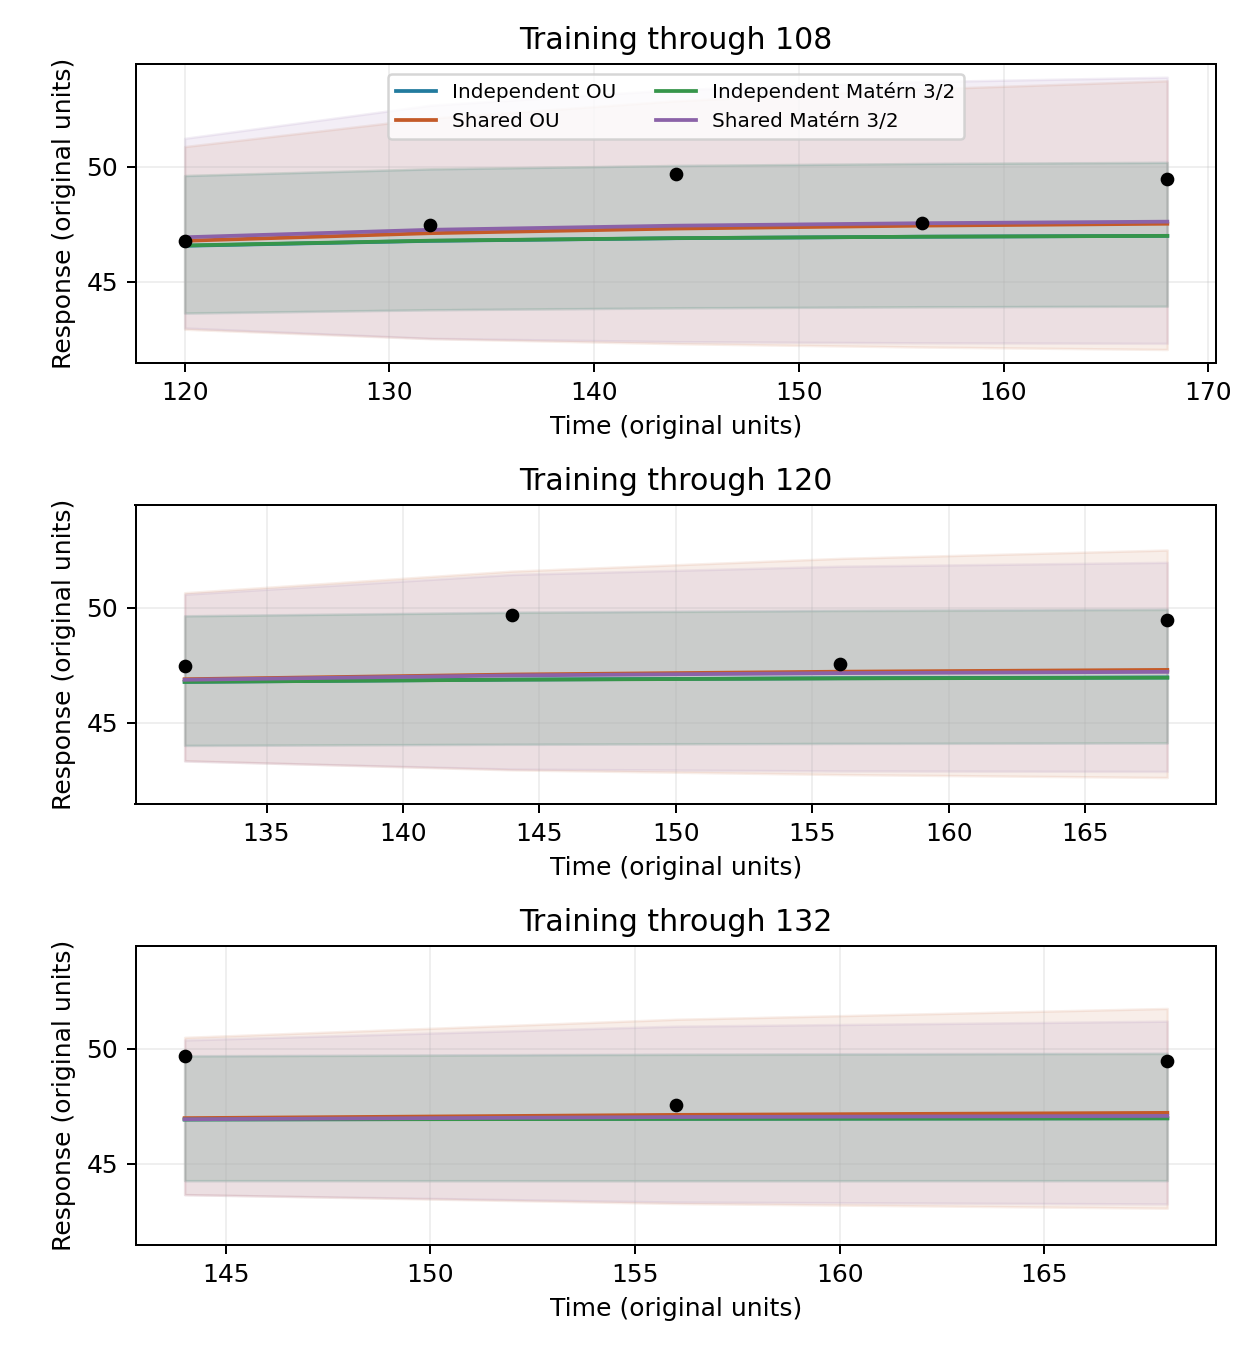
\includegraphics[width=\textwidth]{../results/structural/forecast_comparison.png}
    \caption{Matched structural alternatives, reference priors: trial 1
    predictive means and central 90 percent observation intervals. Black
    points are held-out responses. All reported scores use all three trials.}
    \label{fig:structural-forecast}
\end{figure}
\begin{figure}[htbp]
    \centering
    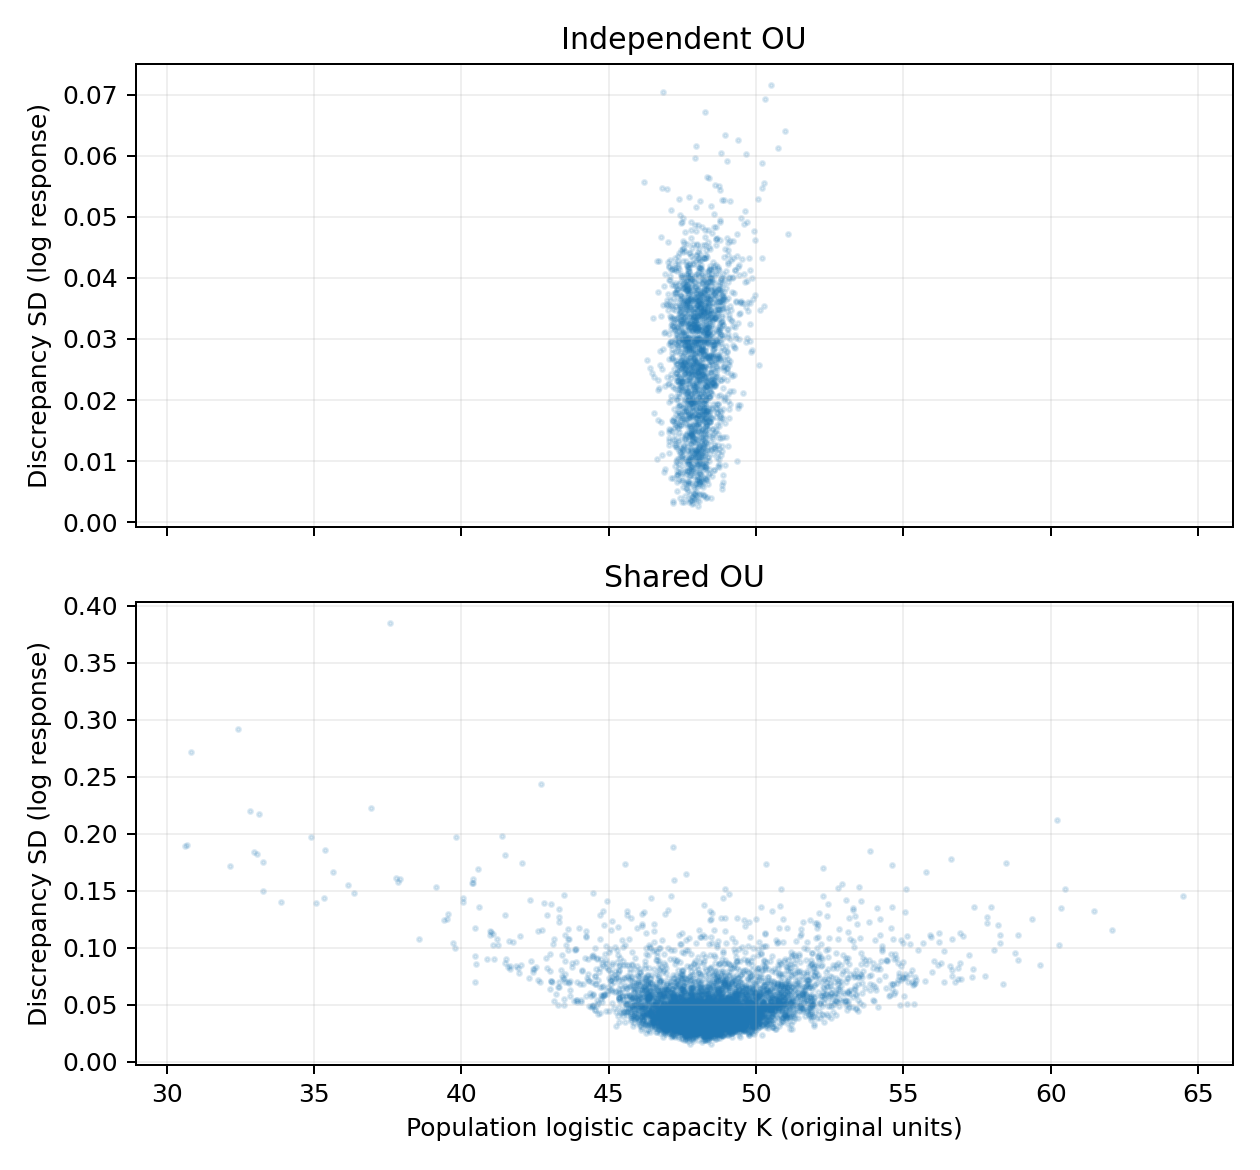
\includegraphics[width=0.9\textwidth]{../results/structural/capacity_discrepancy.png}
    \caption{Full-data reference posterior samples for capacity and discrepancy
    amplitude under independent and shared OU assumptions. The shared model
    allows greater uncertainty in the population capacity.}
    \label{fig:structural-capacity}
\end{figure}
